\documentclass[a4paper, 12pt, titlepage]{report}
\usepackage{minted}
\usepackage[dvipsnames]{xcolor}
\colorlet{LightBlue}{RoyalBlue!20}
\usepackage{graphicx}
\usepackage{fullpage}
\usepackage{float}
\usepackage{amsmath}
\usepackage{booktabs}
\usepackage{multicol}
\usepackage{graphicx}
\usepackage{fullpage}
\usepackage{float}
\usepackage{hyperref}
\usepackage{csquotes}
\usepackage[backend=biber]{biblatex}
\addbibresource{bibfile.bib}
\setlength{\tabcolsep}{18pt}
\renewcommand{\arraystretch}{1.5}
\renewcommand{\chaptername}{Section}
\hypersetup{
    colorlinks=true,
    linkcolor=RoyalBlue,
    filecolor=RoyalBlue,
    urlcolor=RoyalBlue,
    citecolor=RoyalBlue,
}
\begin{document}
\linespread{1.5}
\author{Affaan Muhammad - 33016763\\Joshua Esterhuizen - 30285976}
\title{ITRI625 - Computer Security II\\Metasploit Project Documentation}
\date{Due: October, 19th 2021}
\maketitle
\tableofcontents{}
\chapter{Installation and Setup}
\section{Project files}
The project files can be found on the following GitHub link:\\
\url{https://github.com/AM-ops/MetasploitProject/}
\\\\This was our main code repository. We both have been updating the code as we went along and added details and bug fixes to the project.\\\\
To copy the code to your own machine, follow the following steps:
\begin{enumerate}
\item Make sure Git is installed. If not it can be downloaded from here:\\
\url{https://git-scm.com/}
\item Create an empty directory where the code can be copied to
\item Run the following command:
\begin{minted}
[
frame=lines,
framesep=2mm,
baselinestretch=1.2,
bgcolor=LightBlue,
fontsize=\footnotesize,
]
{Shell}
git clone https://github.com/AM-ops/MetasploitProject.git
\end{minted}
\end{enumerate}
\section{Virtual Environments}
There are multiple advantages of using virtual environments when testing for vulnerabilities and exploits in computer security. The primary reason being we create a layer of separation and abstraction between our host machine and our virtual environments. This 'sand-boxing' allows for analysis of threats in a contained environment.
\subsection{VirtualBox}
We made use of Oracle's VirtualBox software for the virtualisation. This can be downloaded from the following link: \url{https://www.virtualbox.org/wiki/Downloads}\\
Below is a screenshot of the site. We also chose the \texttt{Windows hosts} option to download. Other hosts can also be utilised such as Linux hosts, or OS X hosts.
\begin{figure}[H]
    \centering
    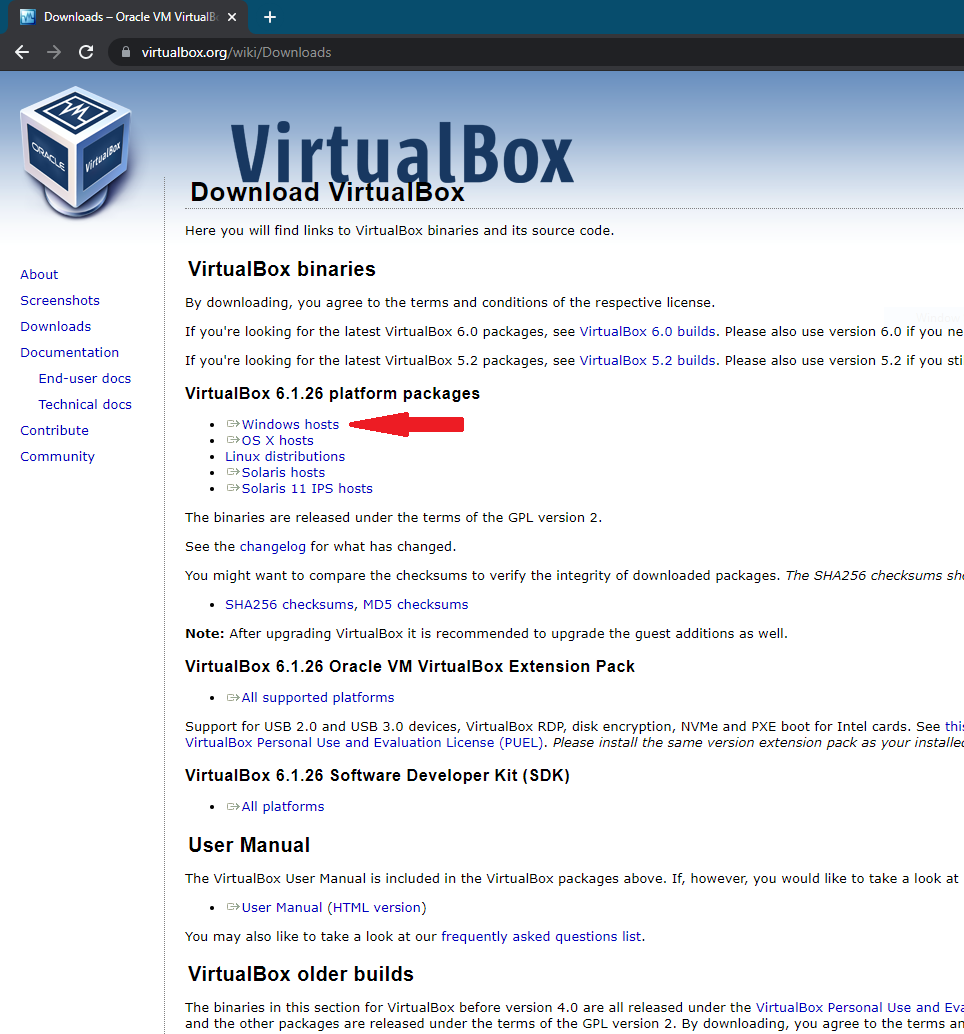
\includegraphics[scale=0.3]{pics/vbmain.PNG}
    \caption{Oracle's VirtualBox Download Page}
\end{figure}
Once the file has been downloaded, open it. Thereafter follow the default prompts of the installation. Below are some figures illustrating this.
\begin{multicols}{2}
\begin{figure}[H]
    \centering
    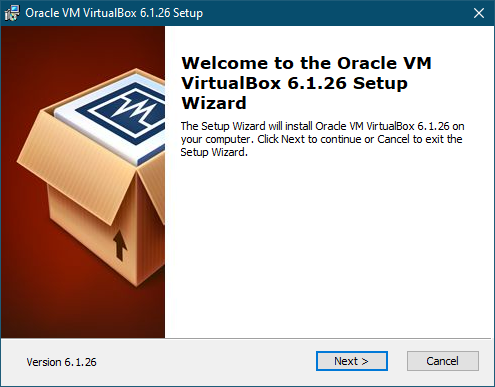
\includegraphics[scale=0.5]{pics/vb1.PNG}
    \caption{Screen 1}
\end{figure}
\begin{figure}[H]
    \centering
    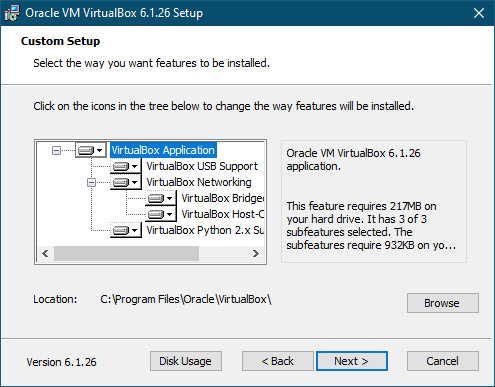
\includegraphics[scale=0.5]{pics/vb2.PNG}
    \caption{Screen 2}
\end{figure}
\end{multicols}
Click on \textbf{Next} for both above screens
\begin{multicols}{2}
\begin{figure}[H]
    \centering
    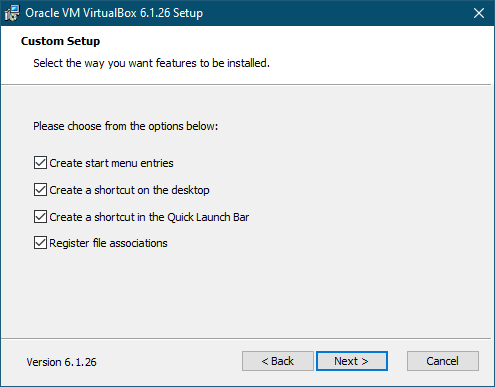
\includegraphics[scale=0.5]{pics/vb3.PNG}
    \caption{Screen 3}
\end{figure}
\begin{figure}[H]
    \centering
    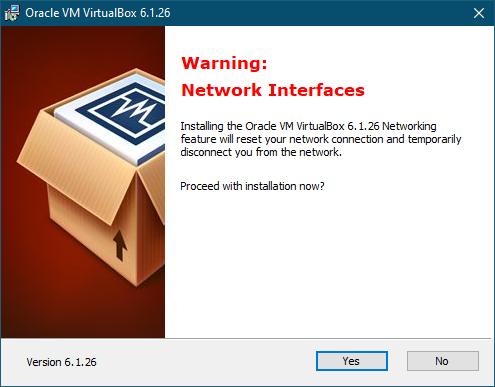
\includegraphics[scale=0.5]{pics/vb4.PNG}
    \caption{Screen 4}
\end{figure}
\end{multicols}
Click on \textbf{Next} for both of the above screens
\begin{multicols}{2}
\begin{figure}[H]
    \centering
    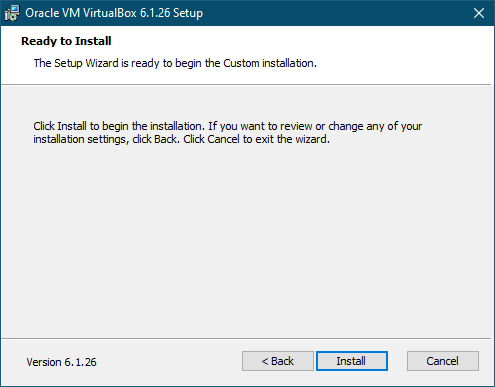
\includegraphics[scale=0.5]{pics/vb5.PNG}
    \caption{Screen 5}
\end{figure}
\begin{figure}[H]
    \centering
    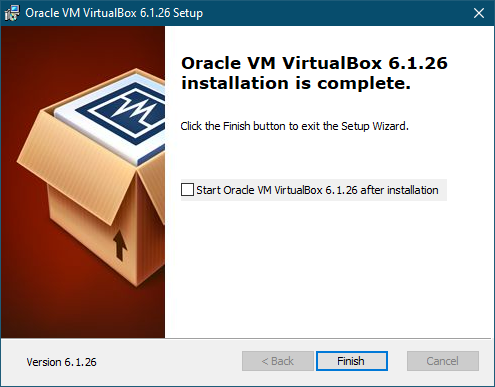
\includegraphics[scale=0.5]{pics/vb6.PNG}
    \caption{Screen 6}
\end{figure}
\end{multicols}
Click on \textbf{Next} and then \textbf{Finish}
\section{Kali Linux}
The next step is to acquire an Operating System for carrying out our Penetration Testing. For this purpose we utilised \texttt{Kali Linux}. The main site for this OS is: \url{https://www.kali.org/}\\\\
According to them they quote the following:
\begin{displayquote}
"\textbf{The Most Advanced Penetration Testing Distribution}\\
\textit{Kali Linux is an open-source, Debian-based Linux distribution geared towards various information security tasks, such as Penetration Testing, Security Research, Computer Forensics and Reverse Engineering.}"
\end{displayquote}
\pagebreak
The main site looks as follows
\begin{figure}[H]
    \centering
    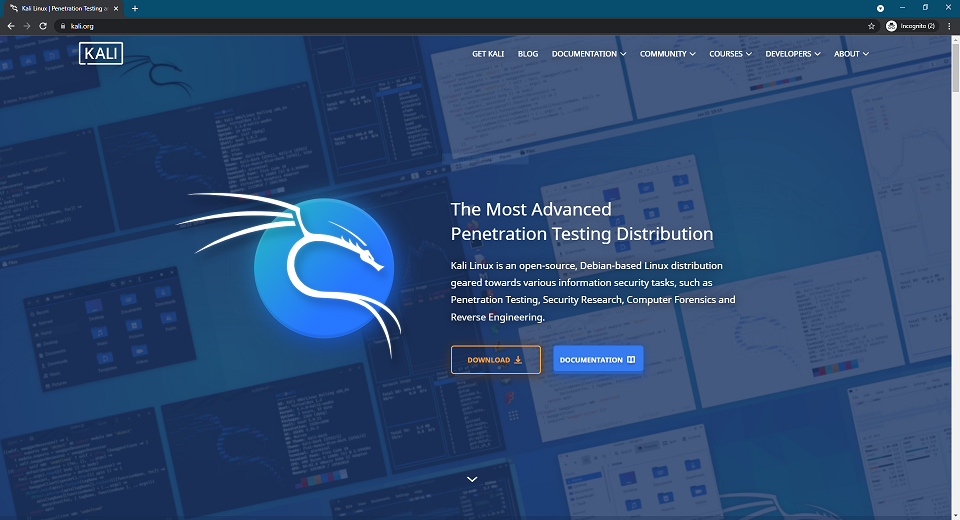
\includegraphics[scale=0.5]{pics/kali.PNG}
    \caption{Kali Linux's Homepage}
\end{figure}
Click on the \texttt{Download} button to see the different options available. Below the options are shown.
\begin{figure}[H]
    \centering
    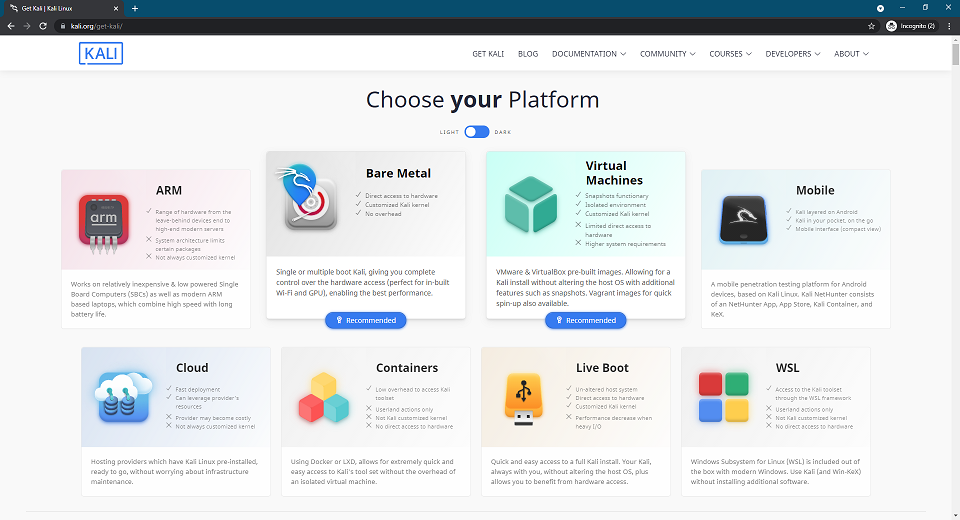
\includegraphics[scale=0.5]{pics/kalidown.PNG}
    \caption{Kali Linux's different download options}
\end{figure}
The option we chose is the \texttt{Virtual Machines} one. Thereafter you are presented with the two options available.
\begin{figure}[H]
    \centering
    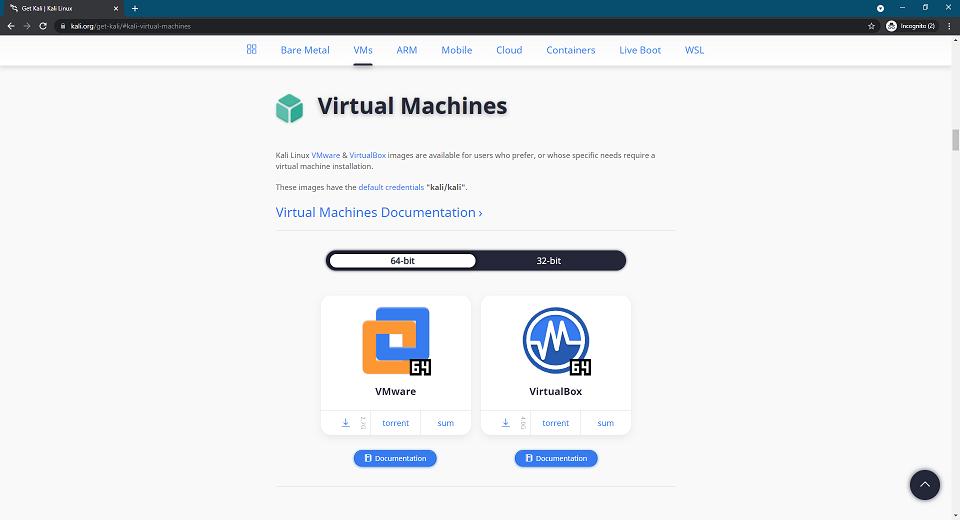
\includegraphics[scale=0.5]{pics/kalivb.PNG}
    \caption{The 2 options for Virtual Machines}
\end{figure}
Select the \texttt{VirtualBox} option and click on the direct download link.\\\\
After the download is completed it is time to set up Kali Linux inside VirtualBox.
\url{https://citizenlab.ca/}
\printbibliography[heading=bibintoc]
\end{document}